\documentclass[a4paper, 11pt, russian]{article}

\usepackage[utf8]{inputenc}
\usepackage[T1, T2A]{fontenc}
\usepackage[english, main = russian]{babel}
\usepackage{graphicx}
\usepackage{natbib}
\usepackage{caption, subcaption}
\usepackage[top=2cm, left=2cm, right=2cm, left=2cm]{geometry}
\usepackage{amsmath} %Для работы с матрицами
\usepackage{ragged2e}
\usepackage{indentfirst}
\parindent 1.27cm 

\newcommand{\jj}{\righthyphenmin=20 \justifying}

\graphicspath{{Images/}}

\captionsetup[figure]{name = Рисунок, labelsep = endash}
\captionsetup[table]{name = Таблица, labelsep = endash, justification=raggedright, singlelinecheck=false}

\begin{document}
    \newcommand\tline[2]{$\underset{\text{#1}}{\text{\underline{\hspace{#2}}}}$}

\begin{titlepage}
	\centering
	{\fontsize{12pt}{5cm}\selectfont \bfseries Министерство образования и науки Российской Федерации} \\ \vspace{0.5cm}
	{\fontsize{7pt}{5cm}\selectfont ФЕДЕРАЛЬНОЕ ГОСУДАРСТВЕННОЕ АВТОНОМНОЕ ОБРАЗОВАТЕЛЬНОЕ УЧРЕЖДЕНИЕ ВЫСШЕГО ПРОФЕССИОНАЛЬНОГО ОБРАЗОВАНИЯ} \\ 
	\vspace{1cm}
	{\fontsize{12pt}{5cm}\selectfont \bfseries САНКТ-ПЕТЕРБУРГСКИЙ УНИВЕРСИТЕТ ИНФОРМАЦИОННЫХ ТЕХНОЛОГИЙ, МЕХАНИКИ И ОПТИКИ} \\ \vspace{1.5cm}

	{\fontsize{14pt}{5cm}\selectfont Кафедра \hspace{1cm} \underline{Систем Управления и Информатики}  \hspace{1cm} Группа \underline{Р3340}} \\ 
	\vspace{2cm}

	{\fontsize{20pt}{5cm}\selectfont \bfseries Лабораторная работа №7} \\
	{\fontsize{20pt}{5cm}\selectfont \bfseries “Анализ точности систем управления”} \\
	{\fontsize{14pt}{5cm}\selectfont Вариант - 2} \\
	\vspace{1.5cm}

	\flushleft

	{Выполнил \hspace{2cm} \underline{Алякин С.П.}\tline{(фамилия, и.о.)}{6.5cm} (подпись)} \\
	\vspace{2cm}

	{Проверил \hspace{2cm} \tline{(фамилия, и.о.)}{9cm} (подпись)} \\
	\vspace{5cm}

	"\underline{\hspace{0.7cm}}"\hspace{0.2cm}\underline{\hspace{2cm}}\hspace{0.2cm}20\underline{ 17 }г. \hspace{2cm} Санкт-Петербург, \hspace{2cm} 20\underline{ 17 }г. \\ \vspace{1cm}

	Работа выполнена с оценкой \hspace{1cm} \underline{\hspace{8cm}} \\ 
	\vspace{1cm}
	Дата защиты "\underline{\hspace{0.7cm}}"\hspace{0.2cm}\underline{\hspace{2cm}}\hspace{0.2cm}20\underline{ 17 }г.
		
\end{titlepage}
    \section*{Цель работы}
    Изучение частотных характеристик типовых динамических звеньев и способов их построения.
    \section*{Исходные данные}
    \begin{table}[h!]
        \flushleft
        \caption{Исходные данные}
        \begin{tabular}{|c|c|c|}
        	\hline
            $k$ & $T$ & $\xi$ \\
            \hline
            2 & 0,5 & 0,15 \\
            \hline
        \end{tabular}
    \end{table}
    \flushleft 
    Сопрягающая частота $\displaystyle{\frac{1}{T}} = 2$\\
    Входной сигнал $g(t) = g_m\sin{\omega t}$\\
    Исследуемые типы звеньев:
    \begin{enumerate}
    	\item Колебательное $W(s) = \displaystyle{\frac{k}{T^2s^2 + 2\xi Ts + 1}}$
        \item Идеальное интегрирующее $W(s) = \displaystyle{\frac{k}{s}}$
        \item Изодромное $W(s) = \displaystyle{\frac{k(1 + Ts)}{s}}$
    \end{enumerate}    
    \clearpage
    \section{Колебательное звено} \parindent 1.27cm \indent 
    Частотная передаточная функция для колебательного звена:
    $$W(j\omega) = W(s)\big|_{s = j\omega} = \frac{k}{1 -T^2\omega^2 + jT\xi\omega} = \frac{k(1 - T^2\omega^2)}{(1 - T^2\omega^2)^2 + (2T\xi\omega)^2} - j\frac{2T\xi\omega k}{(1 - T^2\omega^2)^2 + (2T\xi\omega)^2} \eqno (1)$$
    $$U(\omega) = \frac{k(1 - T^2\omega^2)}{(1 - T^2\omega^2)^2 + (2T\xi\omega)^2} = \frac{2 - 0,5\omega^2}{(1 - 0,25\omega^2)^2 + 0,0225\omega^2} \eqno (2)$$
    $$V(\omega) = -\frac{2T\xi\omega k}{(1 - T^2\omega^2)^2 + (2T\xi\omega)^2} = -\frac{0,3\omega}{(1 - 0,25\omega^2)^2 + 0,0225\omega^2} \eqno (3)$$
    $$A(\omega) = \sqrt{U^2(\omega) + V^2(\omega)} = \frac{k}{\sqrt{(1 - T^2\omega^2)^2 + (2T\xi\omega)^2}} = \frac{2}{\sqrt{(1 - 0,25\omega^2)^2 + 0,0225\omega^2}} \eqno (4)$$
    \begin{equation*}
        \psi(\omega) =
        \begin{cases}
            -\arctg{\displaystyle{\frac{2T\xi\omega}{1 - T^2\omega^2}}} = -\arctg{\displaystyle{\frac{0,15\omega}{1 - 0,25\omega^2}}} &\text{при $\omega \leq \displaystyle{\frac{1}{T}}$}\\
            -\pi - \arctg{\displaystyle{\frac{2T\xi\omega}{1 - T^2\omega^2}}} = -\pi -\arctg{\displaystyle{\frac{0,15\omega}{1 - 0,25\omega^2}}} &\text{при $\omega > \displaystyle{\frac{1}{T}}$}
        \end{cases}
        \eqno (5)
    \end{equation*}
    \begin{figure}[ht!]
        \centering
        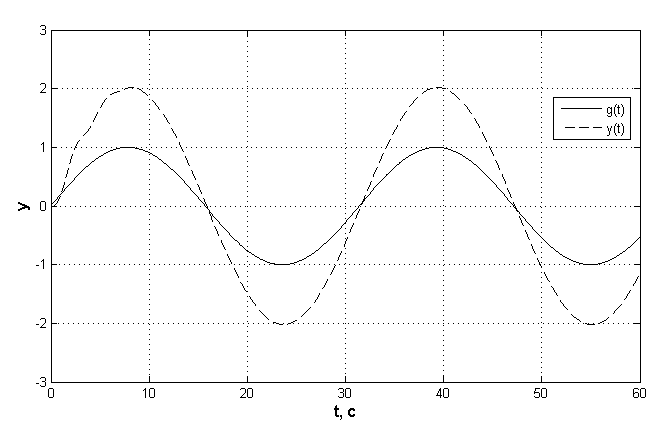
\includegraphics[width = 0.9\textwidth]{oscillatoryLink1}
        \caption{Временная диаграмма колебательного звена}
    \end{figure}
    \begin{table}[ht!]
        \flushleft
        \caption{Данные исследования колебательного звена}
        \begin{tabular}{|c|c|c|c|c|}
        	\hline
            $\omega$ & $\lg{\omega}$ & $A(\omega)$ & $L(\omega)$ & $\psi(\omega)$\\
            \hline
            0,2 & -0,69 & 2,02 & 6,11 & -1,74\\
            \hline
            0,35 & -0,45 & 2,06 & 6,28 & -3,1\\
            \hline
            0,5 & -0,3 & 2,13 & 6,57 & -4,57\\
            \hline
            0,71 & 0,15 & 2,27 & 7,12 & -6,95\\
            \hline
            1 & 0 & 2,61 & 8,33 & -11,31\\
            \hline
            1,41 & 0,15 & 3,67 & 11,29 & -22,81\\
            \hline
            2 & 0,3 & 6,67 & 16,48 & -90\\ %w = 1/T
            \hline
            2,82 & 0,45 & 1,86 & 5,39 & -156,82\\
            \hline
            3,98 & 0,6 & 0,66 & -3,61 & -168,59\\
            \hline
            6,31 & 0,8 & 0,22 & -13,15 & -173,97\\
            \hline
            10 & 1 & 0,08 & 21,94 & -176,42\\
            \hline
        \end{tabular}
    \end{table}
    \newpage
    Частотные и логарифмические частотные характеристики приведены на рисунке 2.
    \begin{figure}[ht!]
        \centering
        \begin{subfigure}[h]{0.48\textwidth}
            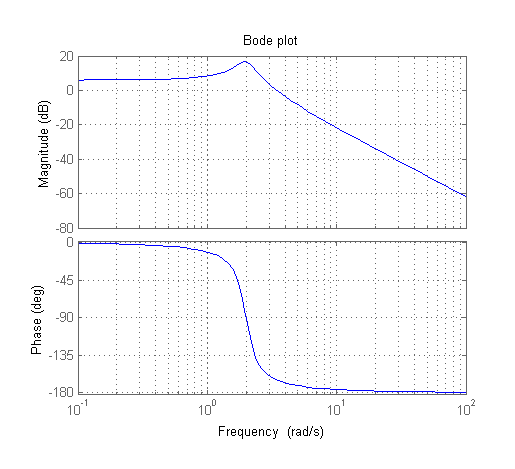
\includegraphics[width = \textwidth]{oscillatoryLinkBode}
            \caption{ЛАЧХ и ЛФЧХ}
        \end{subfigure}
        \hfill
        \begin{subfigure}[h]{0.48\textwidth}
            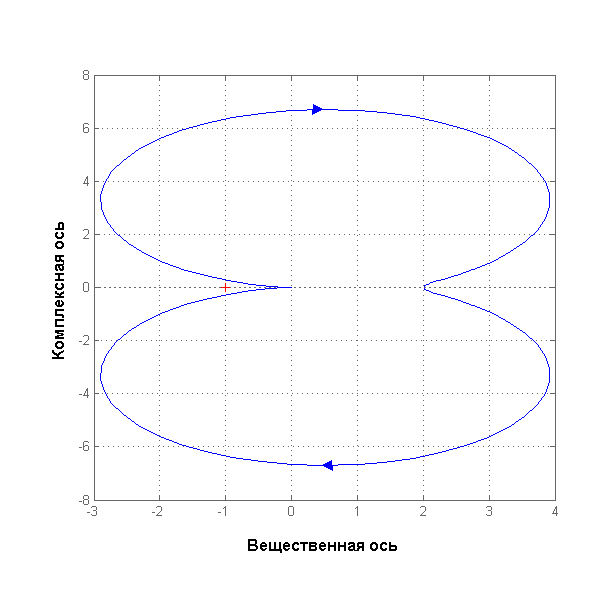
\includegraphics[width = \textwidth]{oscillatoryLinkNyquist}
            \caption{АФЧХ}
        \end{subfigure}
	\end{figure}
	\begin{figure}[ht!]\ContinuedFloat
		\centering
        \begin{subfigure}[h]{0.48\textwidth}
            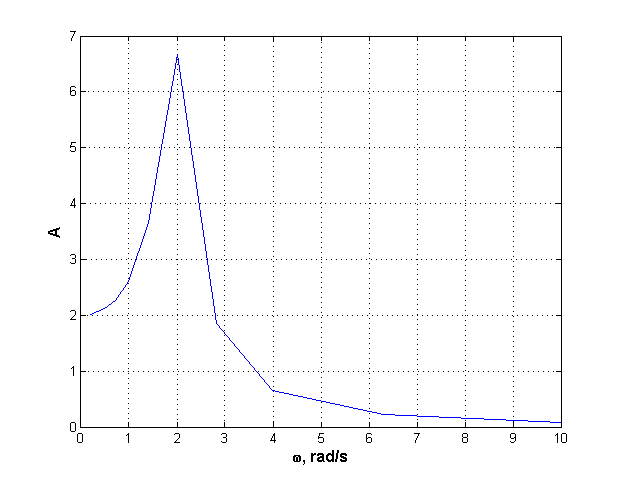
\includegraphics[width = \textwidth]{oscillatoryLinkAFR}
            \caption{АЧХ}
        \end{subfigure}
        \hfill
        \begin{subfigure}[h]{0.48\textwidth}
            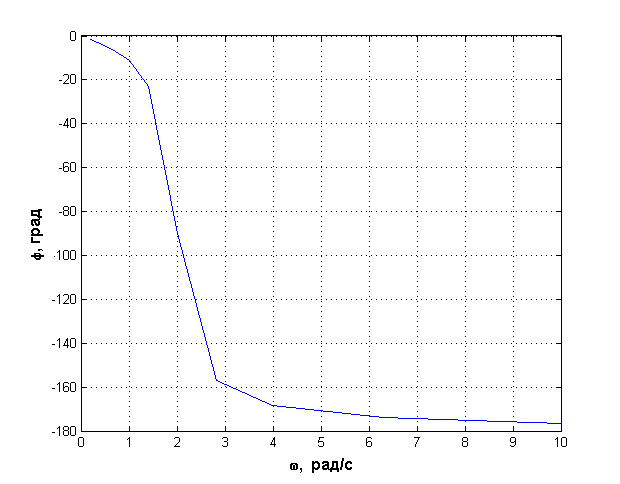
\includegraphics[width = \textwidth]{oscillatoryLinkPFR}
            \caption{ФЧХ}
        \end{subfigure}
        \caption{Характеристики колебательного звена}
    \end{figure}
    \newpage
    Построим асимптотическое ЛАЧХ для данного звена:
    \begin{figure}[ht!]
        \centering
        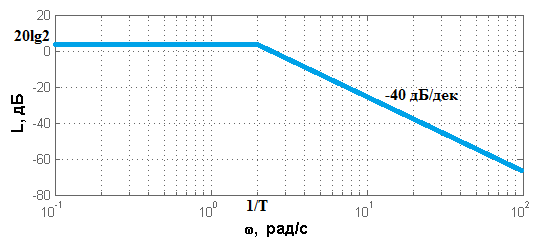
\includegraphics[width = 0.85\textwidth]{oscillatoryLinkAsymp}
        \caption{Асимптотическое ЛАЧХ колебательного звена}
    \end{figure}
    
    \clearpage
    \section{Идеальное интегрирующее звено}
    Частотная передаточная функция для идеального интегрирующего звена:
    $$W(j\omega) = W(s)\big|_{s = j\omega} = \frac{k}{j\omega} = \frac{jk\omega}{-\omega^2} = -j\frac{k}{\omega} \eqno (6)$$
    $$U(\omega) = 0 \eqno (7)$$
    $$V(\omega) = \frac{k}{\omega} = \frac{2}{\omega} \eqno (8)$$
    $$A(\omega) = \frac{2}{\omega} \eqno (9)$$
    $$L(\omega) = 20\lg{A(\omega)} = 20\lg{\frac{2}{\omega}} = 20\lg{2} - 20\lg{\omega} \eqno(10)$$
    $$\psi(\omega) = \arctg{\frac{V(\omega)}{U(\omega)}} = -\arctg{\frac{2}{\omega}} = -\arctg{\infty} = -\frac{\pi}{2} \eqno(11)$$
    \begin{table}[ht!]
        \flushleft
        \caption{Данные исследования идеального интегрирующего звена}
        \begin{tabular}{|c|c|c|c|c|}
        	\hline
            $\omega$ & $\lg{\omega}$ & $A(\omega)$ & $L(\omega)$ & $\psi(\omega)$\\
            \hline
            0,2 & -0,69 & 10 & 20 & -90\\
            \hline
            0,35 & -0,45 & 5,71 & 15,13 & -90\\
            \hline
            0,5 & -0,3 & 4 & 12,04 & -90\\
            \hline
            0,71 & 0,15 & 2,82 & 9 & -90\\
            \hline
            1 & 0 & 2 & 6,02 & -90\\
            \hline
            1,41 & 0,15 & 1,42 & 3,05 & -90\\
            \hline
            2 & 0,3 & 1 & 0 & -90\\ 
            \hline
            2,82 & 0,45 & 0,71 & -2,97 & -90\\
            \hline
            3,98 & 0,6 & 0,5 & -6,02 & -90\\
            \hline
            6,31 & 0,8 & 0,32 & -9,89 & -90\\
            \hline
            10 & 1 & 0,2 & -13,97 & -90\\
            \hline
        \end{tabular}
    \end{table}
    
    Построим асимптотическое ЛАЧХ для интегрирующего звена:
    \begin{figure}[ht!]
        \centering
        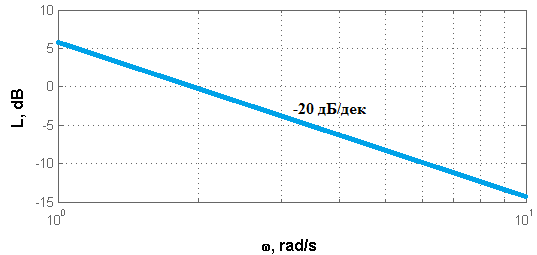
\includegraphics[width = 0.8\textwidth]{integratingLinkAsymp}
        \caption{Асимптотическое ЛАЧХ идеального интегрирующего звена}
    \end{figure}
    \begin{figure}[ht!]
        \centering
        \begin{subfigure}[h]{0.49\textwidth}
            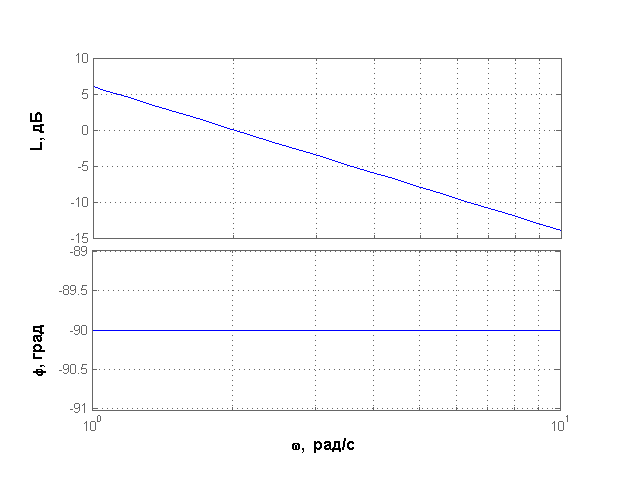
\includegraphics[width = \textwidth]{integratingLinkBode}
            \caption{ЛАЧХ и ЛФЧХ}
        \end{subfigure}
        \hfill
        \begin{subfigure}[h]{0.49\textwidth}
            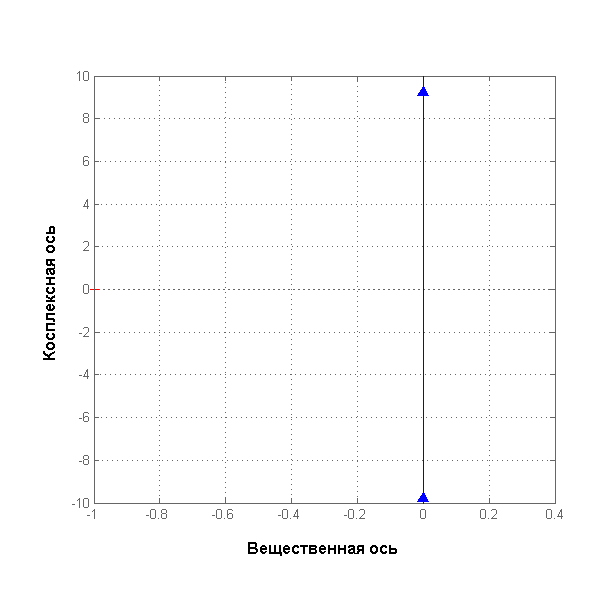
\includegraphics[width = \textwidth]{integratingLinkNyquist}
            \caption{АФЧХ}
        \end{subfigure}
        
        \begin{subfigure}[h]{0.49\textwidth}\ContinuedFloat
            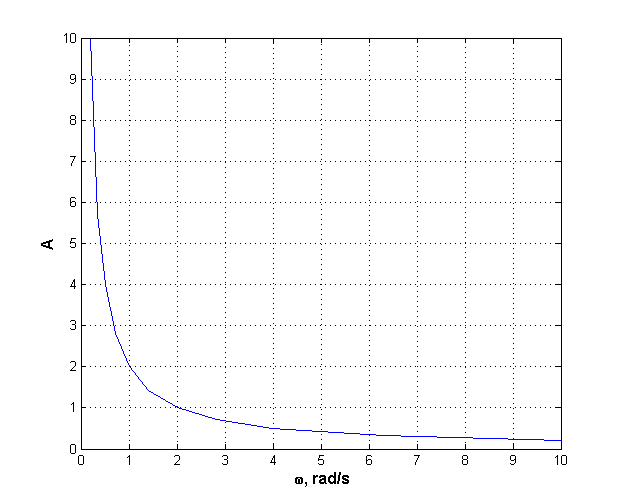
\includegraphics[width = \textwidth]{integratingLinkAFR}
            \caption{АЧХ}
        \end{subfigure}
        \hfill
        \begin{subfigure}[h]{0.49\textwidth}
            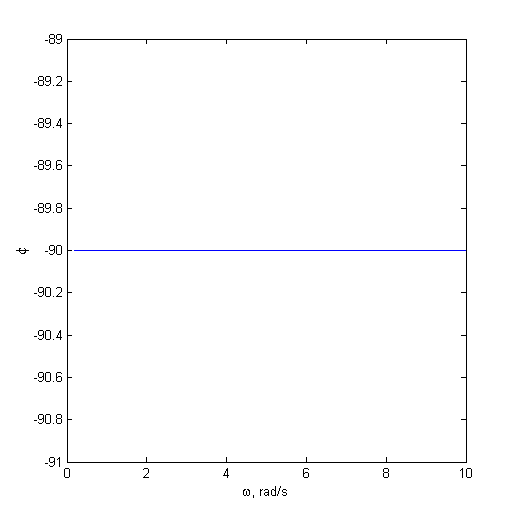
\includegraphics[width = \textwidth]{integratingLinkPFR}
            \caption{ФЧХ}
        \end{subfigure}
        \caption{Характеристики идеального интегрирующего звена}
    \end{figure}
    \clearpage
    \section{Изодромное звено}
    Частотная характеристика для изодромного звена:
    $$W(j\omega) = W(s)\big|_{s = j\omega} = \frac{k(1 + jT\omega)}{j\omega} = \frac{-kT\omega^2 + jk\omega}{-\omega^2} = \frac{kT\omega - jk}{\omega} = kT - j\frac{k}{\omega} \eqno (12)$$
    $$U(\omega) = kT = 1 \eqno (13)$$
    $$V(\omega) = -\frac{k}{\omega} = -\frac{2}{\omega} \eqno (14)$$
    $$A(\omega) = \sqrt{1 + \displaystyle{\frac{4}{\omega^2}}} \eqno (15)$$
    $$L(\omega) = 20\lg{\sqrt{1 + \frac{4}{\omega^2}}} \eqno(16)$$
    $$\psi(\omega) = -\arctg{\frac{2}{\omega}} \eqno (17)$$
    \begin{table}[ht!]
        \flushleft
        \caption{Данные исследования изодромного звена}
        \begin{tabular}{|c|c|c|c|c|}
        	\hline
            $\omega$ & $\lg{\omega}$ & $A(\omega)$ & $L(\omega)$ & $\psi(\omega)$\\
            \hline
            0,2 & -0,69 & 10,05& 20,04& -84,29\\
            \hline
            0,35& -0,45 & 5,8  & 14,12& -80,07\\
            \hline
            0,5 & -0,3  & 4,12 & 12,29& -75,96\\
            \hline
            0,71& 0,15  & 2,99 & 9,51 & -70,46\\
            \hline
            1   & 0     & 2,24 & 7    & -63,43\\
            \hline
            1,41& 0,15  & 1,74 & 4,81 & -54,82\\
            \hline
            2   & 0,3   & 1,41 & 2,98 & -45\\ 
            \hline
            2,82& 0,45  & 1,23 & 1,79 & -35,35\\
            \hline
            3,98& 0,6   & 1,12 & 0,98 & -26,68\\
            \hline
            6,31& 0,8   & 1,05 & 0,42 & -17,59\\
            \hline
            10  & 1     & 1,02 & 0,17 & -11,31\\
            \hline
        \end{tabular}
    \end{table}
    \begin{figure}[ht!]
        \centering
        \begin{subfigure}[h]{0.48\textwidth}
            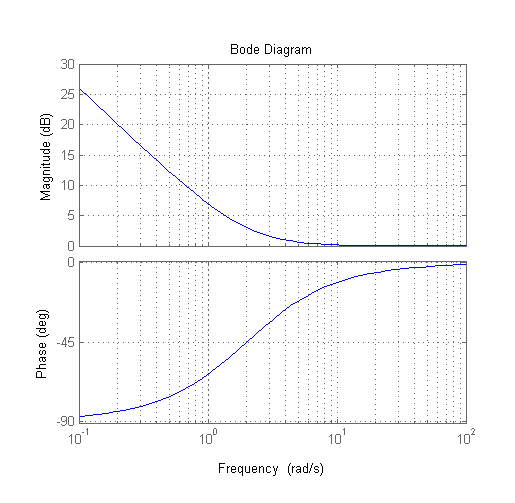
\includegraphics[width = \textwidth]{isodromusLinkBode}
            \caption{ЛАЧХ и ЛФЧХ}
        \end{subfigure}
        \hfill
        \begin{subfigure}[h]{0.48\textwidth}
            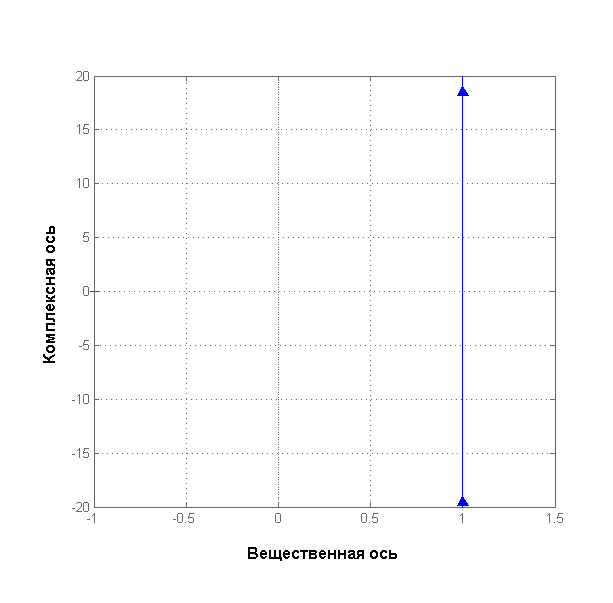
\includegraphics[width = \textwidth]{isodromusLinkNyquist}
            \caption{АФЧХ}
        \end{subfigure}
        
        \begin{subfigure}[h]{0.48\textwidth}
            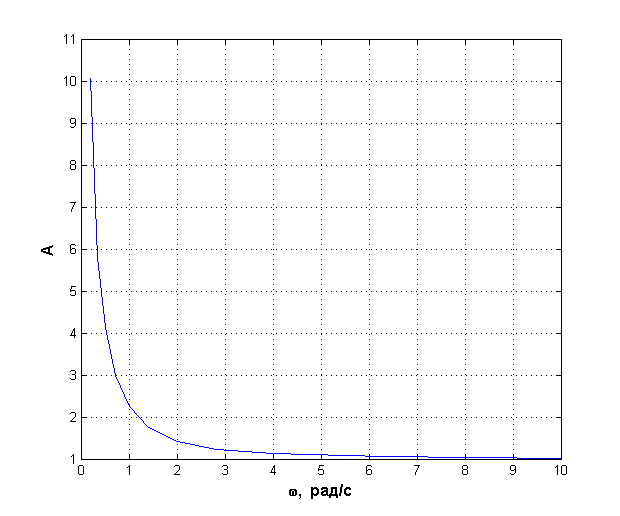
\includegraphics[width = \textwidth]{isodromusLinkAFR}
            \caption{АЧХ}
        \end{subfigure}
        \hfill
        \begin{subfigure}[h]{0.48\textwidth}
            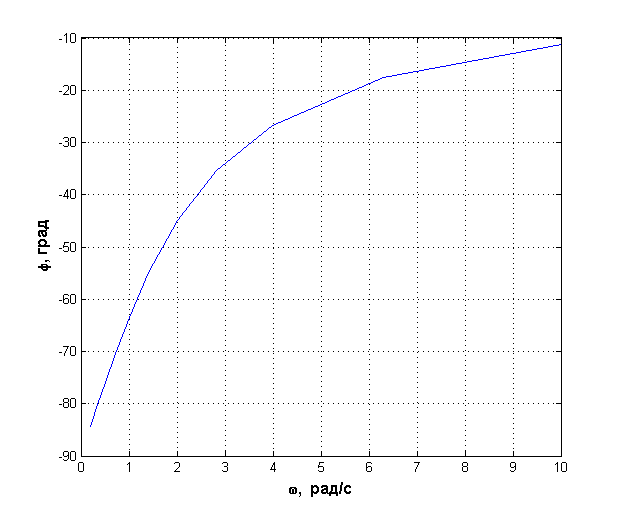
\includegraphics[width = \textwidth]{isodromusLinkPFR}
            \caption{ФЧХ}
        \end{subfigure}
        \caption{Характеристики изодормного звена}
    \end{figure}
    \begin{figure}[ht!]
        \centering
        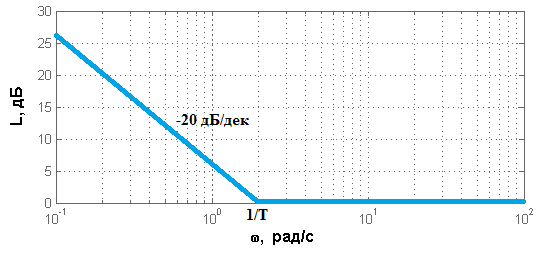
\includegraphics[scale = 0.8]{isodromusLinkAsymp}
        \caption{Асимптотическое ЛАЧХ изодромного звена}
    \end{figure}
    \clearpage
    \section*{Вывод} \jj
    В данной работе были изучены обычные и логарифмические частотные характеристики типовых динамических звеньев, а так же методы построения асимптотических ЛАЧХ. И было доказано, что асимптотические ЛАЧХ сходятся к построенным в ходе математического моделирования, следовательно, могут быть использованы при разработке систем, так как для их построения практически не требуется вычислительная работа.
\end{document}